\section{理论}
在本节中, 我们通过混合分布模型来说明模型的建立过程. 其中加速密度聚类算法是通过一些计算和分析给出的, 堆积速度和叠前时偏移速度模型是通过对聚类中心进行插值估计出来的. 
\subsection{混合分布模型}
\rr{同相轴局部斜率}包含地下反射的几何和速度信息. 有了估计出的\rr{同相轴局部斜率}, 我们可以用简单的一对一映射算子在时域中成像. 从反射时差的经典双曲假设开始: 

\begin{equation}
    t^2(h)=\tau_0^2+\frac{h^2}{V_{\mathrm{NMO}}^2(\tau_0)}
\end{equation}

其中$\tau_0$为双向零偏距走时, $t(h)$代表偏移量$h$处记录的双向走时, $V_{\mathrm{NMO}}(\tau_0)$为叠加速度. 我们将$t(h)$相对于$h$的导数表示为$p_h$(走时斜率):
\begin{equation}
    p_{h}(t, h)=\frac{d t}{d h}=\frac{h}{t V_{\mathrm{NMO}}^{2}\left(\tau_{0}\right)}
\end{equation}
通过上述两个方程, 叠加速度速度$V_{\mathrm{NMO}}(\tau_0)$和零偏距走时$\tau_0$可以被有效的表示出来(\cite{Ottolini1983, Fomel2007}), 如下面的两个公式所示: 
\begin{equation}
    V_{\mathrm{NMO}}\left(\tau_{0}\right)=\sqrt{\frac{h}{t p_{h}(t, h)}}
    \label{equ:3}
\end{equation}
和
\begin{equation}
    \tau_{0}=\sqrt{t^{2}-t p_{h}(t, h) h}
    \label{equ:4}
\end{equation}
为了在每个CMP道集上得到一个稳健的\rr{同相轴局部斜率}估计$p_h$, 我们采用了了PWD(\cite{Fomel2002, Chen2013})算法. 在具体应用中可以将斜率估计算法用其他算法进行替换. 域$\{t,h\}$上的单个CMP道集数据点通过方程(\ref{equ:3})和(\ref{equ:4})映射到零偏距走时和叠加速度域$\{\tau_0,V_{\mathrm{NMO}}\}$. 在偏移点的附近, \rr{同相轴局部斜率}接近零. 因此, 我们不使用零偏移点附近的数据. 与通过图像扭曲的速度图不同的是(\cite{Fomel2007}), 我们不再使用数据点的振幅. 数据点以相等的权重被映射到新的空间中. 对于实际数据的应用, 可以用从估计斜率中得到的局部相干性来分配每个要映射的数据的权重(\cite{Zhang2013}). 
\begin{figure}[htb]
    \centering
    \subfigure[使用随机噪声的人工合成 CMP 道集. \label{fig:1a}]{
        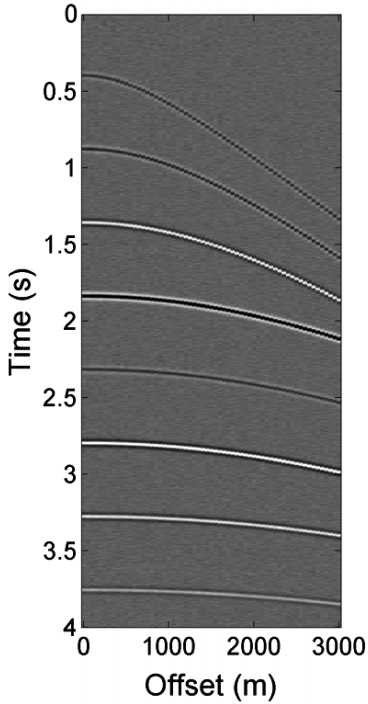
\includegraphics[scale=.2]{1a.png}
    }
    \subfigure[使用 PWD 估计斜率. \label{fig:1b}]{
        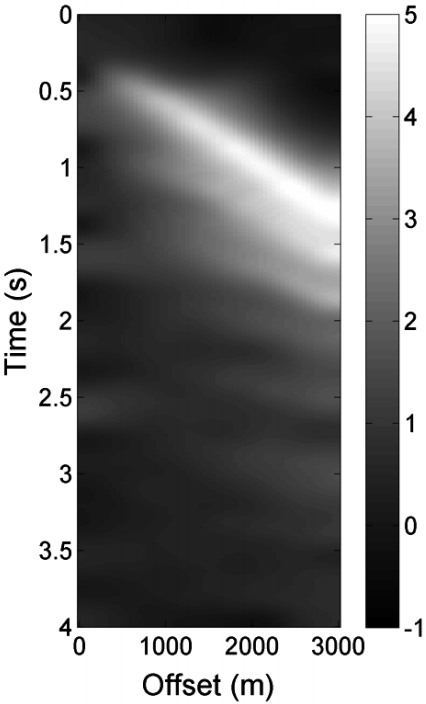
\includegraphics[scale=.2]{1b.png}
    }
    \subfigure[从局部属性映射到局部斜率的结果. \label{fig:1c}]{
        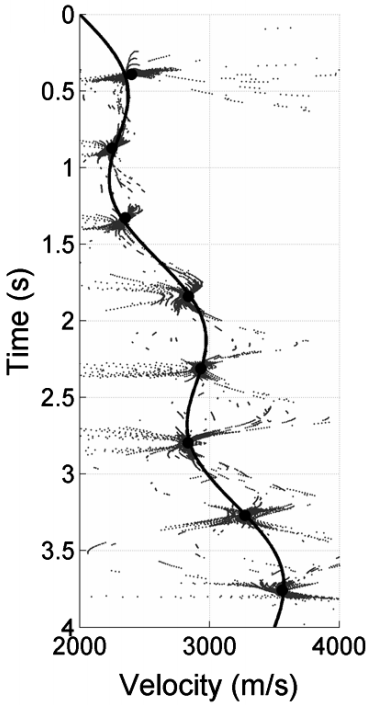
\includegraphics[scale=.2]{1c.png}
    }
    \caption{10dB随机噪声的人工数据示例. \ref{sub@fig:1c} 中, 灰色数据点是映射后的数据, 黑色圆圈是聚类中心, 黑色曲线表示真实速度. 
    }
\end{figure}
图~\ref{fig:1a} 是使用8个收集器的在速度平滑变化的介质中的简单实验. CMP道集的Ricker子波峰值频率为 20 Hz, 接收器的间隔为 50 m, 电缆总长度为 3 km, 时间间隔为4 ms, 总时间为 4 s, 该图是将速度从从 2.0 km∕s开始应用逆动校正获得的. CMP道集中添加了 10dB 的随机高斯噪声. 图~\ref{fig:1b} 描述了PWD估计出的\rr{同相轴局部斜率}. 可以看出, 估计出的\rr{同相轴局部斜率}相当平稳. 图~\ref{fig:1c} 显示了数据点映射到$\{\tau_0,V_{\mathrm{NMO}}\}$空间后的分布. 

需要注意的是, 新空间中的数据点有成簇的性质. 鉴于反射时差的双曲假设可以完全描述反射事件的运动, 并且能完美估计\rr{同相轴局部斜率}, 因此, 新空间中的数据点应该对应一次相同位置上的反射事件. 在面对实际数据时, 双曲假设不能完全描述非平面反射体, 因此, 估计出的斜率永远会有偏差, 一个反射事件会被映射成一簇. 假定双曲假设和斜率估计算法的误差遵循高斯分布, 那么, 一次反射数据的映射结果可以用一个高斯分布来表示, 其期望值为极大似然估计. 对于多与一次反射的情况, 可以直观的引入高斯混合模型. 作为高斯分布的简单线性叠加, 高斯混合模型可以表示更加复杂的密度模型(\cite{Bishop2006}). 高斯混合模型如下: 
\begin{equation}
    P(\mathbf{x})=\sum_{k=1}^{K} a_{k} N_{k}\left(\mathbf{x} \mid \mu_{k}, \sigma_{k}\right)
\end{equation}
其中, $x$为映射数据点在新空间中的位置, $N_{k}\left(\mathbf{x} \mid \mu_{k}, \sigma_{k}\right)$为高斯分布, $x$的期望为$\mu_k$, 标准差为$\sigma_k$, $K$代表单个高斯分布的总数量, $a_k$取混合系数. 分布$P(x)$是联合分布$P(x|x\in N_k)$对所有可能的状态$P(x\in N_k)$的总和, 即
\begin{equation}
    P(\mathbf{x})=\sum_{k=1}^{K} P\left(\mathbf{x} \in N_{k}\right) P\left(\mathbf{x} \mid \mathbf{x} \in N_{k}\right)
\end{equation}
其中$P(x\in N_k)$等于混合系数$a_k$. 通过寻找这$K$个聚类中心, 可以有效地计算出每个高斯分布的期望值$\mu_k$. 

在图~\ref{fig:1c} 中, 黑色圆圈代表聚类中心, 它给出了速度的极大似然解, 黑色曲线为真实的NMO速度. 可以看出, 所有的聚类中心都落在了真实的NMO速度的路径上. 聚类中心的数量为8个, 等于反射体的数量. 因此, 混合分布模型可以有效地解决计算从\rr{同相轴局部斜率}映射的速度值的极大似然解的问题. 
\begin{figure}[htb]
    \centering
    \subfigure[使用随机噪声的人工合成 CMP 道集. \label{fig:2a}]{
        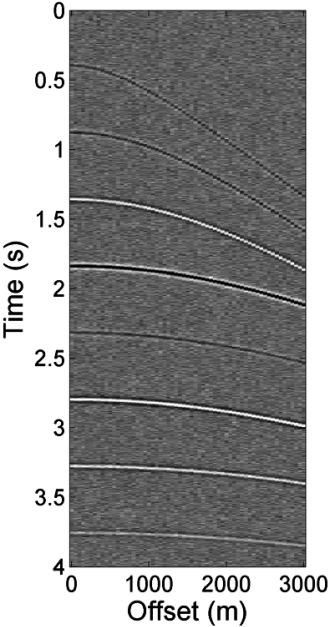
\includegraphics[scale=.2]{2a.png}
    }
    \subfigure[使用 PWD 估计斜率. \label{fig:2b}]{
        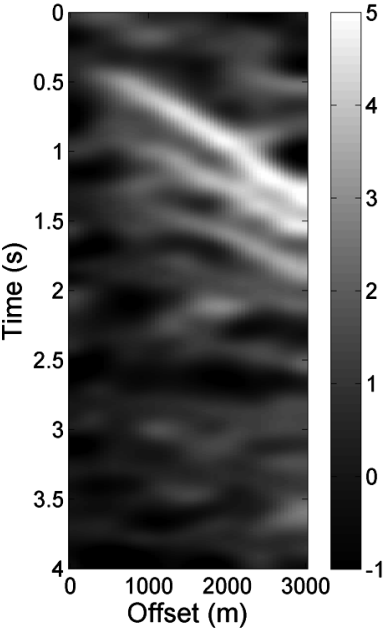
\includegraphics[scale=.2]{2b.png}
    }
    \subfigure[从局部属性映射到局部斜率的结果. \label{fig:2c}]{
        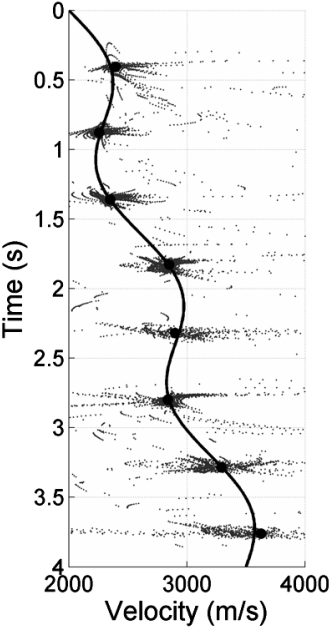
\includegraphics[scale=.2]{2c.png}
    }
    \caption{0dB随机噪声的人工数据示例. }
\end{figure}

估计出的\rr{同相轴局部斜率}的质量会因为噪声和干扰而降低. 图~\ref{fig:2a} 显示了与图~\ref{fig:1a} 中相同的CMP道集, 但添加了不同水平的随机噪声, 其信噪比为0dB. 在这种情况下, 信号的功率等于随机高斯噪声的功率. 图~\ref{fig:2b} 展示了PWD的估计出的\rr{同相轴局部斜率}. 尽管在PWD之前已经使用了带通滤波器来过滤噪声, 但估计出的\rr{同相轴局部斜率}仍受到了强噪声的影响. 图~\ref{fig:2c} 显示了在$\{\tau_0,V_{\mathrm{NMO}}\}$空间中的映射数据点, 直接映射算子给出了被高频振荡污染的部分. 在图~\ref{fig:2c} 中, 黑色圆圈代表聚类中心, 黑色实心曲线是真实的NMO速度. 可以看出, 此时所有的聚类中心仍然与真实NMO速度的路径相吻合, 这证实了聚类中心对\rr{同相轴局部斜率}的估计是稳健的. 
\subsection{加速密度聚类}
在所有用于寻找聚类中心的算法中, k-means可能是应用最广泛的那一个. 为了实施k-means算法, 需要提前知道聚类中心的数量, 但这一先验信息通常难以确定(\cite{Hamerly2004}). (\cite{Wang2012})实现了层次聚类和划分, 以便在储层表征中找到正确的聚类中心数量. 通过带分割和合并的k-means方法(\cite{Muhr2009}), 可以在合理的运行时间内选取出准确的聚类中心数量. (\cite{Lu2014})应用类似的策略来确定浅水中的衍射地震噪声. 在k-means中, 数据点总是被分配到距离最近的中心. 虽然可以用各种距离将其拓展, 但k-means还是几乎不能检测到非球形簇. 

密度聚类(\cite{Rodriguez2014})则更容易应对更一般的数据分布情况. 聚类簇数也更容易确定. 聚类中心被描述为为密度相对高于相邻点, 而且与其他密度较大的中心点距离较大的点. 对于每个数据点$i$, 其局部密度$\rho_i$和其与密度较高的点的最小距离$\sigma_i$是密度聚类中的两个十分重要的参数. 简单的$\rho_i$定义为:
\begin{equation}
    \rho_{i}=\sum_{j} \lambda\left(d_{i j}-d_{c}\right)
\end{equation}
其中, $d_{ij}$为数据点$i$与数据点$j$之间的距离, $d_c$为截止距离, 如果$d_{ij}-d_c<0$, 则$λ = 1$, 否则$λ = 0$. 该算法仅对不同数据点的$\rho_i$敏感, 这意味着其结果对参数于$d_c$是稳健的(\cite{Rodriguez2014}). 而一个数据点到密度较高的点的最小距离$\sigma_i$为: 
\begin{equation}
    \delta_{i}=\min _{j: \rho_{j}>\rho_{i}}\left(d_{i j}\right)
\end{equation}

对于密度最大的点, $\sigma_i$取值为$\max_j(d_{ij})$. 根据$\sigma_i$的定义, 我们可以得出$\sigma_i$只有在全局或局部最大值时才相对较大的. 然后选取局部密度$\rho_i$相对较大、最小距离$\sigma_i$相对较大的点作为聚类中心. 在实际应用中, 我们可以通过$\beta$的快速变化来确定中心, 即$\beta$是$\rho$和$\sigma$的乘积. 确定聚类中心后, 按照局部密度最高到最低的顺序对数据点进行分配. 数据点总是被分配到离其最近的局部密度较高的那一类中. 总的来说, 密度聚类对$N$个数据点的计算复杂度为$O(N^2)$, 详细复杂度分析见附录~\ref{Appendix:A}. 即使对于单个CMP道集, 在典型的1000个时间样本和100个源-接收器对的情况下, 也可能有105个数据点. 这使得密度聚类算法在实际数据应用也不太合适. 










